\documentclass[
  11pt,
  a4paper,
  twoside,
  german,
  headsepline,
  footnosepline=false,
  automark,
  normalheadings,
  openany,
  cleardoubleplain,
  abstracton, 
  idxtotoc,
  liststotoc,
  bibtotoc,
  BCOR8mm
]{scrreprt}

% The following is needed in order to make the code compatible
% with both latex/dvips and pdflatex.
\ifx\pdftexversion\undefined
\usepackage[dvips]{graphicx}
\else
\usepackage[pdftex]{graphicx}
\DeclareGraphicsRule{*}{mps}{*}{}
\fi

\usepackage{ae}
\usepackage{aecompl}
\usepackage{amsfonts}
\usepackage{amsmath}
\usepackage{amssymb}
\usepackage[ngerman]{babel}
\usepackage{calc}
\usepackage{color}
\usepackage{enumerate}
\usepackage{fancybox}
\usepackage{fancyvrb}
\usepackage{float}
\usepackage[T1]{fontenc}
\usepackage{graphicx}
\usepackage{hyperref}
\usepackage[utf8]{inputenc}
\usepackage{mdwlist}
\usepackage[numbers]{natbib}
\usepackage{scrdate}
\usepackage{scrtime}
\usepackage{scrpage2}
\usepackage{tabularx}
\usepackage{forloop}
\usepackage[font={small}]{caption}
\usepackage[font={footnotesize}]{subcaption}

\usepackage{algpseudocode}
\usepackage{algorithmicx}

\renewcommand{\algorithmicrequire}{\textbf{Eingabe:}}
\renewcommand{\algorithmicensure}{\textbf{Ausgabe:}}

\usepackage{todonotes}

\usepackage{user}

\usepackage{listings}

\usepackage{caption}
\usepackage{subcaption}

\allowdisplaybreaks

\usepackage{color}
\definecolor{string}{rgb}{0.16,0,1}
\definecolor{identifier}{rgb}{0.25,0.5,0.5}
\definecolor{keyword}{rgb}{0.5,0,0.5}

\lstset{
  numberstyle=\scriptsize\ttfamily\color{gray},
  basicstyle=\scriptsize\ttfamily,
  columns=fullflexible,
  showstringspaces=false,
  numbers=left,
  stepnumber=1,
  breaklines=true
}

\lstdefinelanguage{XSD}
{
  morestring=[b]",
  stringstyle=\color{string},
  identifierstyle=\color{identifier},
  keywordstyle=\color{keyword},
  morekeywords={xmlns,version,type,default,name,value,base,minOccurs,maxOccurs,
    use, targetNamespace,elementFormDefault,encoding}
}

\newcommand{\writtenby}[1]{%
  \todo[nolist,noline,color=yellow!50]{#1}\noindent%
}

\newcommand{\qedsymbol}{\ensuremath{\blacksquare}}

% Mark a piece of text as surname. Will render the name in all capitals and
% withing an mbox (prevent word breaking).
\newcommand{\surname}[1]{\mbox{\textsc{#1}}}

\pagestyle{scrheadings}
\setkomafont{pagehead}{\small\scshape}

\setcounter{tocdepth}{3}

\fussy

\newtheorem{bsp}{Beispiel}[chapter]
\newtheorem{satz}{Satz}[chapter]

\makeatletter
\renewcommand{\env@cases}[1][@{}l@{\quad}l@{}]{%
  \let\@ifnextchar\new@ifnextchar
  \left\lbrace
  \def\arraystretch{1.2}%
  \array{#1}%
}
\makeatother

\newcommand{\code}[1]{\mbox{\texttt{#1}}}

\newlength{\elasticfigurewidth}
\newcommand{\elasticfigure}[2]{%
  \begin{figure}[H]%
    \centering%
    \settowidth{\elasticfigurewidth}{\includegraphics{#1}}%
    \setlength{\elasticfigurewidth}{\minof{\elasticfigurewidth}{\textwidth}}%
    \includegraphics[width=\elasticfigurewidth]{#1}%
    \caption{#2}%
  \end{figure}%
}

\newcommand{\unit}[1]{\ensuremath{\,\mathrm{#1}}}

\hyphenation{
  ab-ge-schwächt
  an-sons-ten
  Ä-qui-va-lenz-en
  auf-zu-wer-ten
  aus-schlie-ßen
  be-stimmt
  be-trach-te-ten
  Bild-aus-schnitt
  Dreh-win-kel
  ent-spre-chen-de
  er-zeugt
  Farb-ko-die-rung
  ge-dreht
  Hel-lig-keits-un-ter-schied
  Hel-lig-keits-zu-wei-sung
  Ini-ti-ali-sie-rung
  Kan-ten-ope-ra-tor
  ma-the-ma-tisch-en
  Me-tho-de
  mi-ni-mal-er
  Pi-xel-wer-ten
  Scan-line-ver-fahr-ens
  zu-sätz-lich-e
}



\begin{document}

\renewcommand{\figurename}{Abb.}

\newcommand{\dcsubject}{Teamorientierte Projektarbeit}
\newcommand{\dctitle}{Entwurf und Implementation von Verfahren zum Auffinden und Lesen von Strichcodes in Videodaten}
\newcommand{\dcsubtitle}{~}

\newcommand{\dcauthornameewie}{Erik Wienhold}
\newcommand{\dcauthornameriren}{René Richter}
\newcommand{\dcauthoremailewie}{ewie@hrz.tu-chemnitz.de}
\newcommand{\dcauthoremailriren}{riren@hrz.tu-chemnitz.de}
\newcommand{\dcauthors}{%
    René Richter \normalsize\texttt{riren@hrz.tu-chemnitz.de} \\
    Erik Wienhold \normalsize\texttt{ewie@hrz.tu-chemnitz.de} \\
}
\newcommand{\dcdate}{\today} 

\newcommand{\dcplace}{Chemnitz}
\newcommand{\dcuni}{Technische Universität \dcplace}
\newcommand{\dcdepart}{Informatik}
\newcommand{\dcprof}{Medieninformatik}

\newcommand{\dcpruefer}{}
\newcommand{\dcadvisor}{Robert Manthey}

\newcommand{\dckeywords}{}

\hypersetup{%
    pdftitle    = {\dctitle},
    pdfsubject  = {\dcsubject, \dcdate},
    pdfauthor   = {\dcauthornameriren \dcauthoremailriren \dcauthornameewie
    \dcauthoremailewie},
    %
    pdfkeywords = {\dckeywords},
    pdfcreator  = {pdfTeX with Hyperref and Thumbpdf},
    pdfproducer = {LaTeX, hyperref, thumbpdf},
}

\titlehead{
    \vspace*{-1.5cm}
    \usekomafont{sectioning}\mdseries
    \begin{center}
        \raisebox{-1ex}{
\includegraphics[scale=1.4]{img/TUC_deutsch_einzeile_CMYK}}\\
        \hrulefill \\[1em]
        {\Large\dcdepart}\\[0.5em]
        \dcprof
    \end{center}
    \vspace*{1.5cm}
}

\subject{\bf\Huge\dcsubject}


\title{\sf\Large
    \dctitle
    \\
    \dcsubtitle
}

\author{%
    \dcauthornameriren \\
    \texttt\dcauthoremailriren
    \and
    \dcauthornameewie \\
    \texttt\dcauthoremailewie
}

\date{\dcplace, den \dcdate}

\publishers{
    {\parbox{\textwidth-8em}{
        \begin{tabbing}
            {\bf Betreuer:}\quad\=\kill
            {\bf Prüfer:}   \>\dcpruefer\\
            {\bf Betreuer:} \>\dcadvisor
        \end{tabbing}
    }}
}

\lowertitleback{
\textbf{\dcauthornameriren\quad\dcauthornameewie}\\
\dctitle\\
\dcsubject,~\dcdepart\\
\dcuni,~\ifcase\month\or
  Januar\or Februar\or März\or April\or Mai\or Juni\or
    Juli\or August\or September\or Oktober\or November\or Dezember\fi
    ~\number\year
}

\maketitle

%\thispagestyle{empty}
%\null\vfil
%\begin{center}
%\usekomafont{sectioning}\textbf{Danksagung}
%\vspace{-.5em}\vspace{\parsep}
%%
%% TODO
%%
%\end{center}
%\par\vfil\null
%\cleardoubleemptypage
%
%\def\abstractname{Abstract}
%\begin{abstract}
%%
%% TODO
%%
%\end{abstract}

\cleardoubleemptypage
\pagenumbering{roman}
%\pdfbookmark{Inhaltsverzeichnis}{Inhaltsverzeichnis}
\tableofcontents

\cleardoublepage
\markboth{Abbildungsverzeichnis}{Abbildungsverzeichnis}
\listoffigures

\cleardoublepage
\markboth{Tabellenverzeichnis}{Tabellenverzeichnis}
\listoftables

%\renewcommand{\listalgorithmname}{Algorithmenverzeichnis}
%\cleardoublepage
%\addcontentsline{toc}{chapter}{Algorithmenverzeichnis}
%\listofalgorithms

%\cleardoublepage
%\addcontentsline{toc}{chapter}{Abkürzungsverzeichnis}
%\markboth{Abk"urzungsverzeichnis}{Abk"urzungsverzeichnis}
%\def\listacronymname{Abk"urzungsverzeichnis}
%\printglosstex(acr)

\cleardoublepage
\pagenumbering{arabic}
\setcounter{page}{1}


\listoftodos

%\manualmark
%\markboth{Literaturverzeichnis}{Literaturverzeichnis}
\bibliographystyle{user}
\bibliography{literature}
\cleardoublepage

\chapter*{Selbstständigkeitserklärung}

Hiermit erklären wir, daß wir die vorliegende Arbeit
selbstständig angefertigt, nicht anderweitig zu Prüfungszwecken vorgelegt und
keine anderen als die angegebenen Hilfsmittel verwendet haben. Sämtliche 
wissentlich verwendeten Textausschnitte, Zitate oder Inhalte anderer Verfasser 
wurden ausdrücklich als solche gekennzeichnet.\\[2ex]
\dcplace, den \dcdate\\[10ex]
\begin{tabular}{p{5cm} p{5cm}}\hline
\footnotesize \dcauthornameriren &
\footnotesize \dcauthornameewie
\end{tabular}

\chapter{Einführung}
\writtenby{\dcauthornameriren}%

\section{Aufgabenstellung}
Die Aufgabe ist es, Strichcodes in Videostreams zu finden, zu extrahieren und zu dekodieren.
Dabei soll eine freie Bibliothek für die Strichcodeerkennung gefunden und genutzt werden.
Die Bilddaten sind möglicherweise dunkel und unscharf.
Außerdem können die Strichcodes auf den Bildern in unterschiedlichster Verfassung (schattiert, rotiert, teils übermalt oder sogar über 2 Frames verteilt) sein.
Diese Probleme sollen Beachtung finden und später mit einem Testset von Strichcodebildern überprüft werden.
Dabei wird erwartet, dass Code und Vorgehensweise ausführlich dokumentiert sind.


\section{Motivation}
In der heutigen Gesellschaft haben Strichcodes immer größere Bedeutung. Nicht nur in der Wirtschaft, sondern auch im alltäglichen Leben haben viele Menschen mit ihnen zu tun. Sie können sogar bereits mit Handys gescannt und ausgelesen werden, was auch oft für Werbezwecke benutzt wird. Die Erkennung der Codes ist dabei zwar bereits gut entwickelt, aber die Bildqualität kann oft die Lesbarkeit verringern. Daher ist es sinnvoll die Strichcodefindung, in Bildern und Videos, und die Bildaufbereitung, für Bilder von schlechter Qualität und unter schlechten Umständen aufgenommenen Bildern, zu verbessern.


\chapter{Grundlagen}
\writtenby{\dcauthornameewie}%
Im Folgenden sollen die diversen bildtechnischen Operationen beschrieben werden, die die Grundlage für die von uns entwickelten bzw. implementierten Verfahren bilden.

\section{Graustufen}
\label{sec:grayscale}
\writtenby{\dcauthornameewie}%
Im Allgemeinen liegen Bilddaten in Farbe vor.
Sind für die Analyse jedoch Bildstrukturen entscheidend, welche sich durch Helligkeitunterschiede ergeben, so ist es nötig diese Helligkeitsinformation aus den Farbbildern zu extrahieren.

Zunächst ist es entscheiden, in welchem Format die Bilder vorliegen, d.h. wie die Farbinformation kodiert ist.
Die zwei gängigsten Formate sind RGB und YCbCr.
RGB kodiert Farbwerte mit 3 Komponenten die den Farbkanälen Rot~(R), Grün~(G) und Blau~(B) entsprechen.
Im Gegensatz dazu stellt YCbCr die Farbinformation mit den 3 Komponenten Helligkeit~(Y), Blau-Gelb-Chrominanz~(Cb) sowie Rot-Grün-Chrominanz~(Cr).
YCbCr findet Anwendung in JPEG/JFIF~\cite{jfif} zur Farbkodierung.

Liegen die Bilddaten in YCbCr vor, da z.B. mit Videos in MPEG gearbeitet wird, bietet es sich an die kodierte Helligkeit~$Y$ direkt zu verwenden, da diese sich an der Helligkeitswahrnehmung des menschlichen Auges orientiert.

Liegt jedoch RGB vor, so muss die Helligkeit explizit ermittelt werden.
Zum einen kann $Y$ nach folgender Formel~\cite[2.5.1]{itu/rec/601} berechnet werden.
\begin{equation}
  Y = K_R R + (1 - K_R - K_B) G + K_B B
\end{equation}
Die Faktoren $K_R$ und $K_B$ sind in den beiden Standards ITU-R BT.601 (SDTV) und ITU-R BT.709 (HDTV) definiert.
%
\begin{itemize}
\item ITU-R BT.601: $K_R=0.299,~K_B=0.114$ \cite[2.5.1]{itu/rec/601}
\item ITU-R BT.709: $K_R=0.2126,~K_B=0.0722$ \cite[4]{itu/rec/709}
\end{itemize}
%
Soll die Konvertierung aber möglichst schnell erfolgen wird auch auf eine einfachere Variante zurückgegriffen\footnote{\href{https://code.google.com/p/zxing/source/browse/trunk/core/src/com/google/zxing/RGBLuminanceSource.java?spec=svn2633&r=2394\#57}{RGBLuminanceSource.java r2394 L57 (code.google.com/p/zxing)}}, welche die Komponente~$G$, im Vergleich zu $R$ und $B$, doppelt gewichtet.
Diese Gewichtung erfolgt auch in allen Digitalkameras deren CCD-Sensor als \textsc{Bayer}-Matrix aufgebaut ist.
\begin{equation}
  Y = \frac{1}{4} R + \frac{1}{2} G + \frac{1}{4}B
\end{equation}
Liegen die Werte $R$, $G$ und $B$ als positive ganze Zahlen vor, kann die Formel durch 3 Additionen sowie 1 Rechtsshift im Binärsystem umgesetzt werden, da die Faktoren allesamt 2er-Potenzen sind.
Siehe Anhang \ref{annex:proof-division} für einen Beweis.
\begin{equation}
  Y = (R + G + G + B) >\!\!> 2
\end{equation}


\section{Dilation}
\writtenby{\dcauthornameewie}%
% Erosion und Dilation, Öffnen und Schliessen
% aus Voss & Süße 1991
Die Dilatation ist eine morphologische Operation um Strukturen eines Bildes zu vergrößern.
Bei die Dilation eines Grauwertbildes wird jedem Pixel der Maximalwert aller Pixel innerhalb einer gewissen Umgebung zugewiesen \cite[3.5]{steinmueller2008}.
Zur Beschreibung der Umgebung dient ein Strukturelement $X$ fester Größe und Form (z.B. ein 3$\times$3 Quadrat), welches mit seinem Mittelpunkt $(0,0)$ über dem betrachteten Pixel platziert wird.
\begin{equation}
  (I\oplus X)(x,y)= \max \left\{ I(x+u,y+v) \;\middle|\; (u,v) \in X \right\} \quad X \subseteq \mathbb{Z}^2
\end{equation}
Eine Dilation findet Anwendung um Bildstrukturen zu verstärken und zusammenzufassen \cite[3.1]{steinmueller2008}.
Es können aber nur Bildstrukturen zusammengefasst werden sofern das Strukturelement groß genug ist um Zwischenräume zu überbrücken.

\begin{figure}[H]
  \label{fig:dilation}
  \centering
  \begin{subfigure}{0.49\linewidth}
    \centering
    
\includegraphics[width=0.5\textwidth]{img/basics/dilation/before}
    \caption{Ausgangsbild (100$\times$100 Pixel)}
  \end{subfigure}
  \begin{subfigure}{0.49\linewidth}
    \centering
    
\includegraphics[width=0.5\textwidth]{img/basics/dilation/after}
    \caption{Dilation mit einem 3$\times$3-Strukturelement}
  \end{subfigure}
  \caption{Beispiel einer Dilation eines Grauwertbildes}
\end{figure}

\section*{Kantenerkennung}

Kanten in einem Bild zeigen sich durch abrupte Helligkeitsänderungen zwischen benachbarten Pixeln.
Um die Helligkeitsänderung für jedes Pixel zu bestimmen muss der Gradient der Helligkeitsfunktion $\nabla I$ eines Bildes berechnet werden.
Das gängigste Verfahren zur Gradientenbestimmung ist die Faltung des Bildes $I$ mit einer Faltungsmatrix $K$ (auch genannt Kernel).
  \[ (I\circ K)(x,y) =
       \sum_{(u,v)\in m\times n}
       I\left(x+u-\frac{m}{2},y+v-\frac{n}{2}\right)K_{u,v}
       \quad K\in\mathbb{R}^{m\times n} \]
Die Berechnung eines einzelnen Gradientenbildes reicht jedoch nicht aus um alle Kanten eines Bildes zu erfassen, da die Faltungsmatrix nur Helligkeitsänderungen entlang einer Dimension erfasst.
Deshalb ist ein zweites Gradientenbild unter Verwendung einer Faltungsmatrix, die Helligkeitsänderungen entlang einer zweiten Dimension erfasst, erforderlich.
In der Regel nutzt man dafür die Transponierte der ersteren Faltungsmatrix.
Der Gradient der Helligkeitsfunktion ergibt sich dann aus
  \[ \nabla I(x,y) = \sqrt{(I \circ K_X)(x,y)^2 + (I \circ K_Y)(x,y)^2} \]

\subsection*{Sobel-Operator}
Eine der häufigsten Faltungsmatrizen ist der \textsc{Sobel}-Operator.
Dieser funktioniert für unsere Anwendung recht gut, ist jedoch anfällig für Bildrauschen.
  \[ K_X = \begin{vmatrix}
       -1 & -2 & -1 \\
        0 &  0 &  0 \\
        1 &  2 &  1
     \end{vmatrix}
     \quad
     K_Y = K_X^\top = \begin{vmatrix}
       -1 & 0 & 1 \\
       -2 & 0 & 2 \\
       -1 & 0 & 1
     \end{vmatrix} \]

\subsection*{Roberts-Operator}
Der \textsc{Roberts}-Operator \cite{DBLP:books/garland/Roberts63} war eine der ersten Faltungsmatrizen die zur Kantenerkennung in technischen Strichzeichnungen verwendet wurde.
Da die Matrix $K_X$ identisch mit ihrer Transponierten ist verwendet man für die zweite Dimension eine Matrix $K_Y$ deren Spalten vertauscht wurden.
  \[ K_X = \begin{vmatrix}
       1 &  0 \\
       0 & -1
     \end{vmatrix}
     \quad
     K_Y = \begin{vmatrix}
        0 & 1 \\
       -1 & 0
     \end{vmatrix} \]

\section*{Segmentierung}

Die Segmentierung findet Anwendung bei der Klassifizierung von Bildelementen.
Dabei wird jedes Pixel anhand eines Kriteriums einer Klasse zugeordnet.
Ein simples Verfahren ist dabei die Verwendung eines Schwellwertes.
  \[ C_I^{(n)}(x,y) = \begin{cases}[c@{\quad}r@{}c@{}l@{}]
       0      &              & \;I(x,y) & \;<    t_1     \\
       1      & t_1     \leq & \;I(x,y) & \;<    t_2     \\
       \vdots &              &   \vdots &                \\
       n-2    & t_{n-2} \leq & \;I(x,y) & \;<    t_{n-1} \\
       n-1    &              & \;I(x,y) & \;\geq t_{n-1}
     \end{cases} \]
Eine der häufigsten Anwendungen ist die Einteilung eines Bildes in zwei Klassen.
Für gewöhnlich ist dies eine Einteilung des Bildes in Vorder- und Hintergrund.
  \[ C_I^{(2)}(x,y) = \begin{cases}
       0 & I(x,y) <    t \\
       1 & I(x,y) \geq t
     \end{cases} \]
Die Berechnung des Schwellwerts $t$ ist dabei entscheidend über die Qualität der Segmentierung, d.h. dass Bildelemente korrekt klassifiziert werden.

\subsection*{Schwellwertbestimmung}
\todo[author=Erik,inline]{Schwellwertbestimmung}

\paragraph{Mittelwert}
Nutzt den Mittelwert der Helligkeit aller Bildpunkte als Schwellwert.
\todo[author=Erik]{Mittelwert Vor- \& Nachteile}

\paragraph{Otsu's Method}
\textsc{Otsu}'s Method ist ein histogrammbasiertes Verfahren, dass eine bimodale Helligkeitsverteilung\footnote{Eine bimodale Helligkeitsverteilung besitzt zwei Maxima die den Helligkeitswerten des Hintergrund bzw. Vordergrund entsprechen. Der optimale Schwellwert liegt im Tal zwischen den Maxima.} voraussetzt.
Der Algorithmus sucht den Schwellwert, der die Varianz innheralb der beiden Klassen minimiert.

\paragraph{Balanced Histogram Thresholding}
Das Balanced Histogram Thresholding erwartet, wie \textsc{Otsu}'s Method, eine bimodale Helligkeitsverteilung.
Das Verfahren ermittelt den Schwellwert derart, dass dieser das Histogramm in zwei gleich "`schwere"' Hälften teilt.
Als Maß für das Gewicht einer Hälfte dient die Summe der absoluten Häufigkeiten aller Klassen der betrachteten Hälfte.
Von der schwereren Häfte werden solange Klassen entfernt bis nur noch eine Klasse betrachtet wird, welche dem gesuchten Schwellwert entspricht.

\subsection*{Schwellwertanwendung}
\todo[author=Erik,inline]{Schwellwertanwendung}

\paragraph{global}
Der Schwellwert wird für das gesamte Bild einmalig berechnet und auf alle Bildpunkte angewandt.
Die Verwendung eines einzelnen Schwellwertes für das gesamte Bild funkioniert nur sofern das Bild gleichmäßtig Belichtet ist.
Ansonsten kann es vorkommen, dass Bildteile die zu gering belichtet sind unterhalb des Schwellwertes liegen und somit als Hintergrund klassifiziert werden.

\paragraph{lokal}
Unterteilt das Bild in disjunkte Regionen und ermittelt jeweils einen eigenen Schwellwert, mit dem der jeweilige Bereich segmentiert wird.
Die negativen Effekte des globalen Thresholding auf das Gesamtbild werden vermieden, können innerhalb einer Region aber dennoch auftreten.
Wodurch es an den Regionsgrenzen zu unterschiedlichen Klassifikationen kommen kann.

\paragraph{dynamisch}
Ermittelt für jeden Bildpunkt einen Schwellwert unter Betrachtung der Umgebung des Bildpunktes.
Anhand des Schwellwertes wird der Bildpunkt einer Klasse zugeordnet.
Vermeidet die Fehler durch ein ungleiche Beleuchtung, wenn eine Pixelumgebung gewählt werden kann, die einer gleichmäßigen Beleuchtung unterliegt.


\section{Connected-Components-Labeling}
\label{sec:connected-components}
\writtenby{\dcauthornameewie}%
Um zusammenhängende Bildstrukturen zu erfassen verwendet man das sogenannte Connected-Components-Labeling.
Dabei wird jeder Bildpunkt genau einer Menge zugeordnet welche je eine Komponente zusammenhängenger Bildpunkte repräsentiert.
Zwei Bildpunkte hängen zusammen, wenn diese benachbart sind und den gleichen Wert besitzen.
Für die Nachbarschaft gibt es verschiedene Modelle.
%
{
\setlength{\labelsep}{\textwidth}
\setlength{\leftmargini}{1.5em}
\begin{description}
\item[4-Konnektivität] betrachtet für ein Pixel~$(x,y)$ die 4 Pixel~$(x\pm1,y)$ und~$(x,y\pm1)$
\item[8-Konnektivität] betrachtet für ein Pixel~$(x,y)$ neben den 4 Pixel der 4-Konnektivität zusätzlich noch die 4 Pixel~$(x\pm1,y\pm1)$
\end{description}
}
%
\begin{figure}[H]
  \centering
  \begin{subfigure}{0.3\columnwidth}
    \centering
    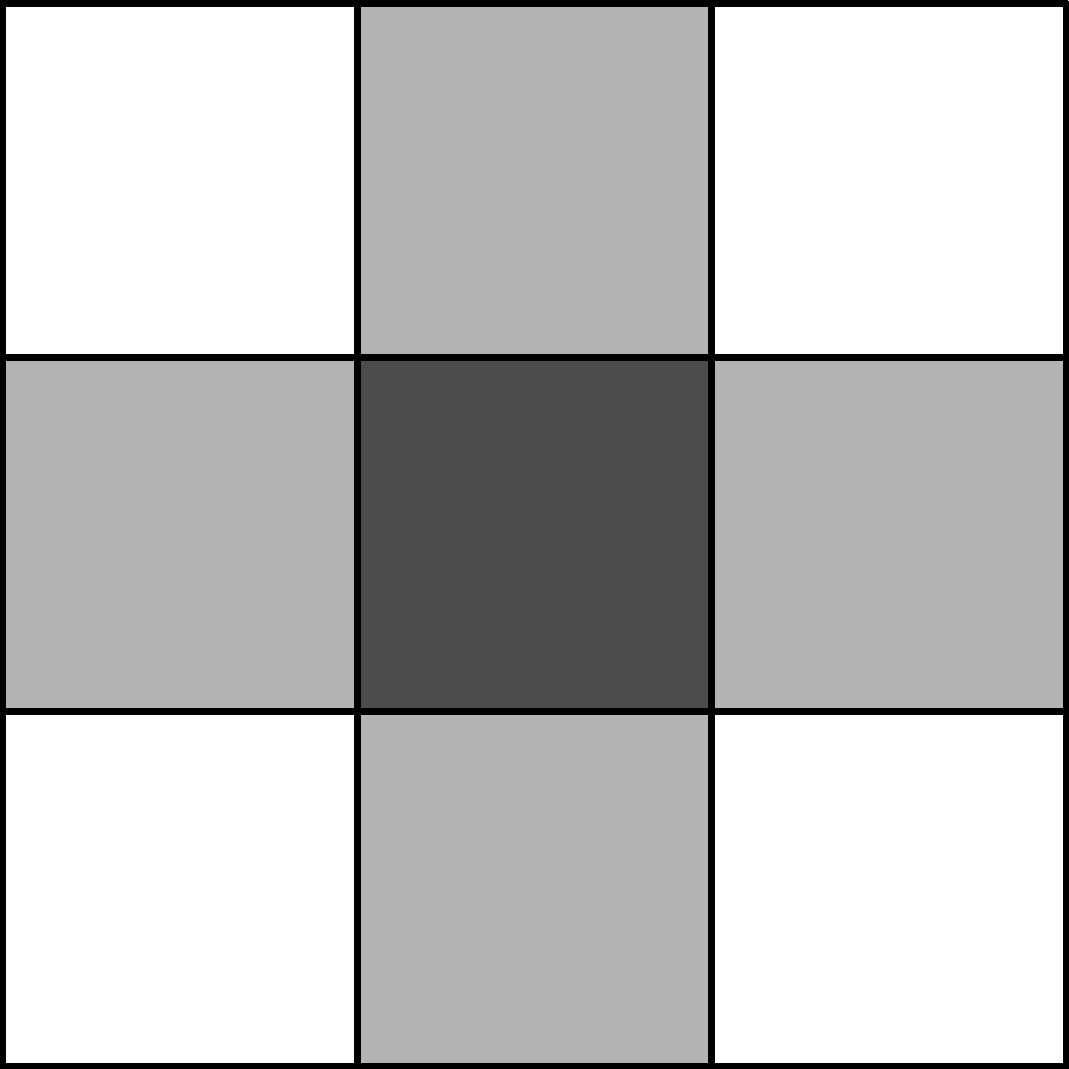
\includegraphics[width=0.5\columnwidth]{img/basics/connected-compontents/4-connectivity}
    \caption{4-Konnektivität}
  \end{subfigure}
  \begin{subfigure}{0.3\columnwidth}
    \centering
    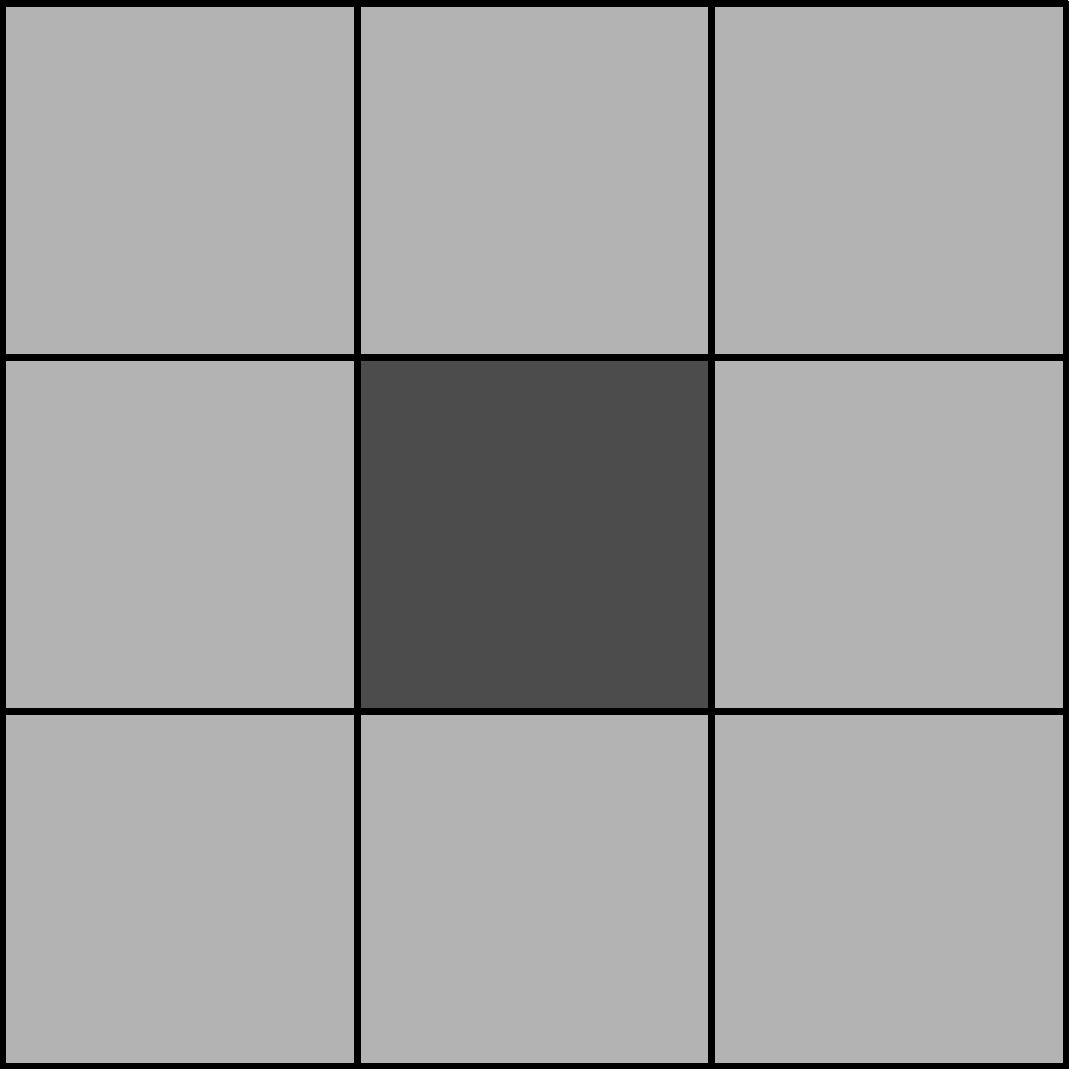
\includegraphics[width=0.5\columnwidth]{img/basics/connected-compontents/8-connectivity}
    \caption{8-Konnektivität}
  \end{subfigure}
  \caption[Vergleich von Pixelnachbarschaften]{Vergleich von Pixelnachbarschaften, mit dem betrachteten Pixel markiert in Dunkelgrau und den Pixeln der Nachbarschaft in Hellgrau.}
\end{figure}
%
Je mehr Pixel als Nachbarschaft herangezogen werden, desto größer können die zusammenhängenden Komponenten ausfallen, da es mehr Möglichkeiten gibt in denen zwei Pixel als verbunden gelten.

Das Connected-Component-Labeling ist realisierbar mittels eines Scanlineverfahrens~\cite[S.~69--75]{compvis2001}, d.h. jede Bildzeile wird, mit der oberen Zeile~($y=0$) beginnend, pixelweise von links~($x=0$) nach rechts verarbeitet.
Jedes Pixel wird auf Verbundenheit mit seinen Nachbarn~(4-Konnektivität) oberhalb~($y-1$) und links~($x-1$) geprüft.
Unterscheidet sich der Wert des aktuellen Pixels von den betrachteten Nachbarn so wird diesem ein neues Label zugewiesen.
Besitzt das Pixel hingegen den Wert mindestens eines Nachbarn so wird das Label des Nachbarn zugewiesen.
Besitzen mehrere Nachbarn den gleichen Wert aber unterschiedliche Label, so werden diese Label als äquivalent markiert.
Die erste Bildzeile und -spalte müssen gesondert initialisert werden, da diese keine Nachbarn oberhalb bzw. links besitzen.
Sind alle Pixel verarbeitet, müssen Labeläquivalenzen aufgelöst werden, sodass Pixeln mit äquivalenten Label ein gemeinsames Label zugewiesen werden kann. Zum Erfassen der Äquivalenzen eignet sich die UnionFind-Datenstruktur.
%
\begin{figure}[H]
  \centering
  \begin{subfigure}[t]{0.327\columnwidth}
    \centering
    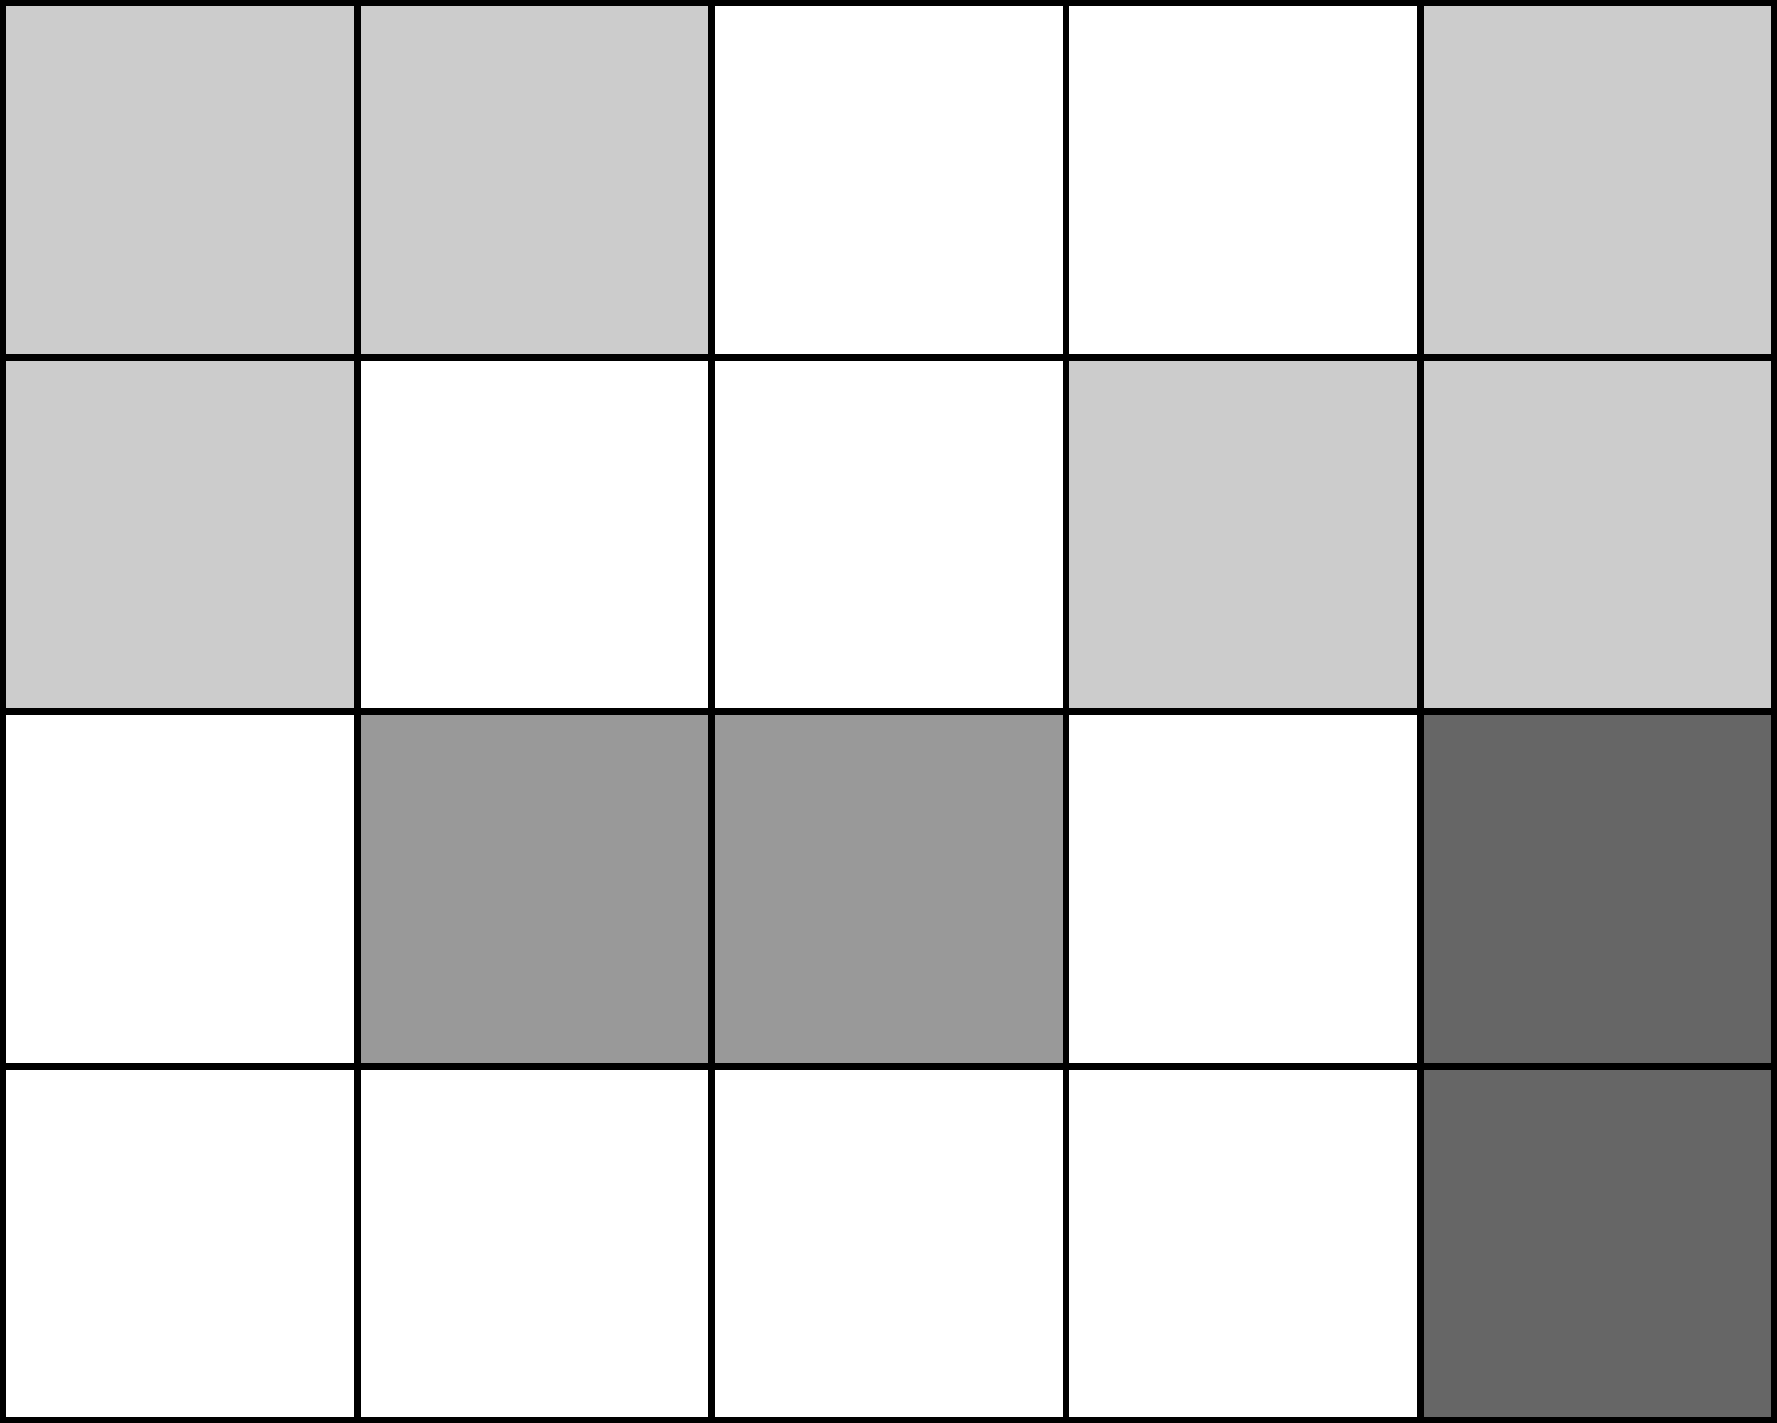
\includegraphics[width=\columnwidth]{img/basics/connected-compontents/labeling-1}
    \caption{Ausgangsgrafik}
  \end{subfigure}
  \begin{subfigure}[t]{0.327\columnwidth}
    \centering
    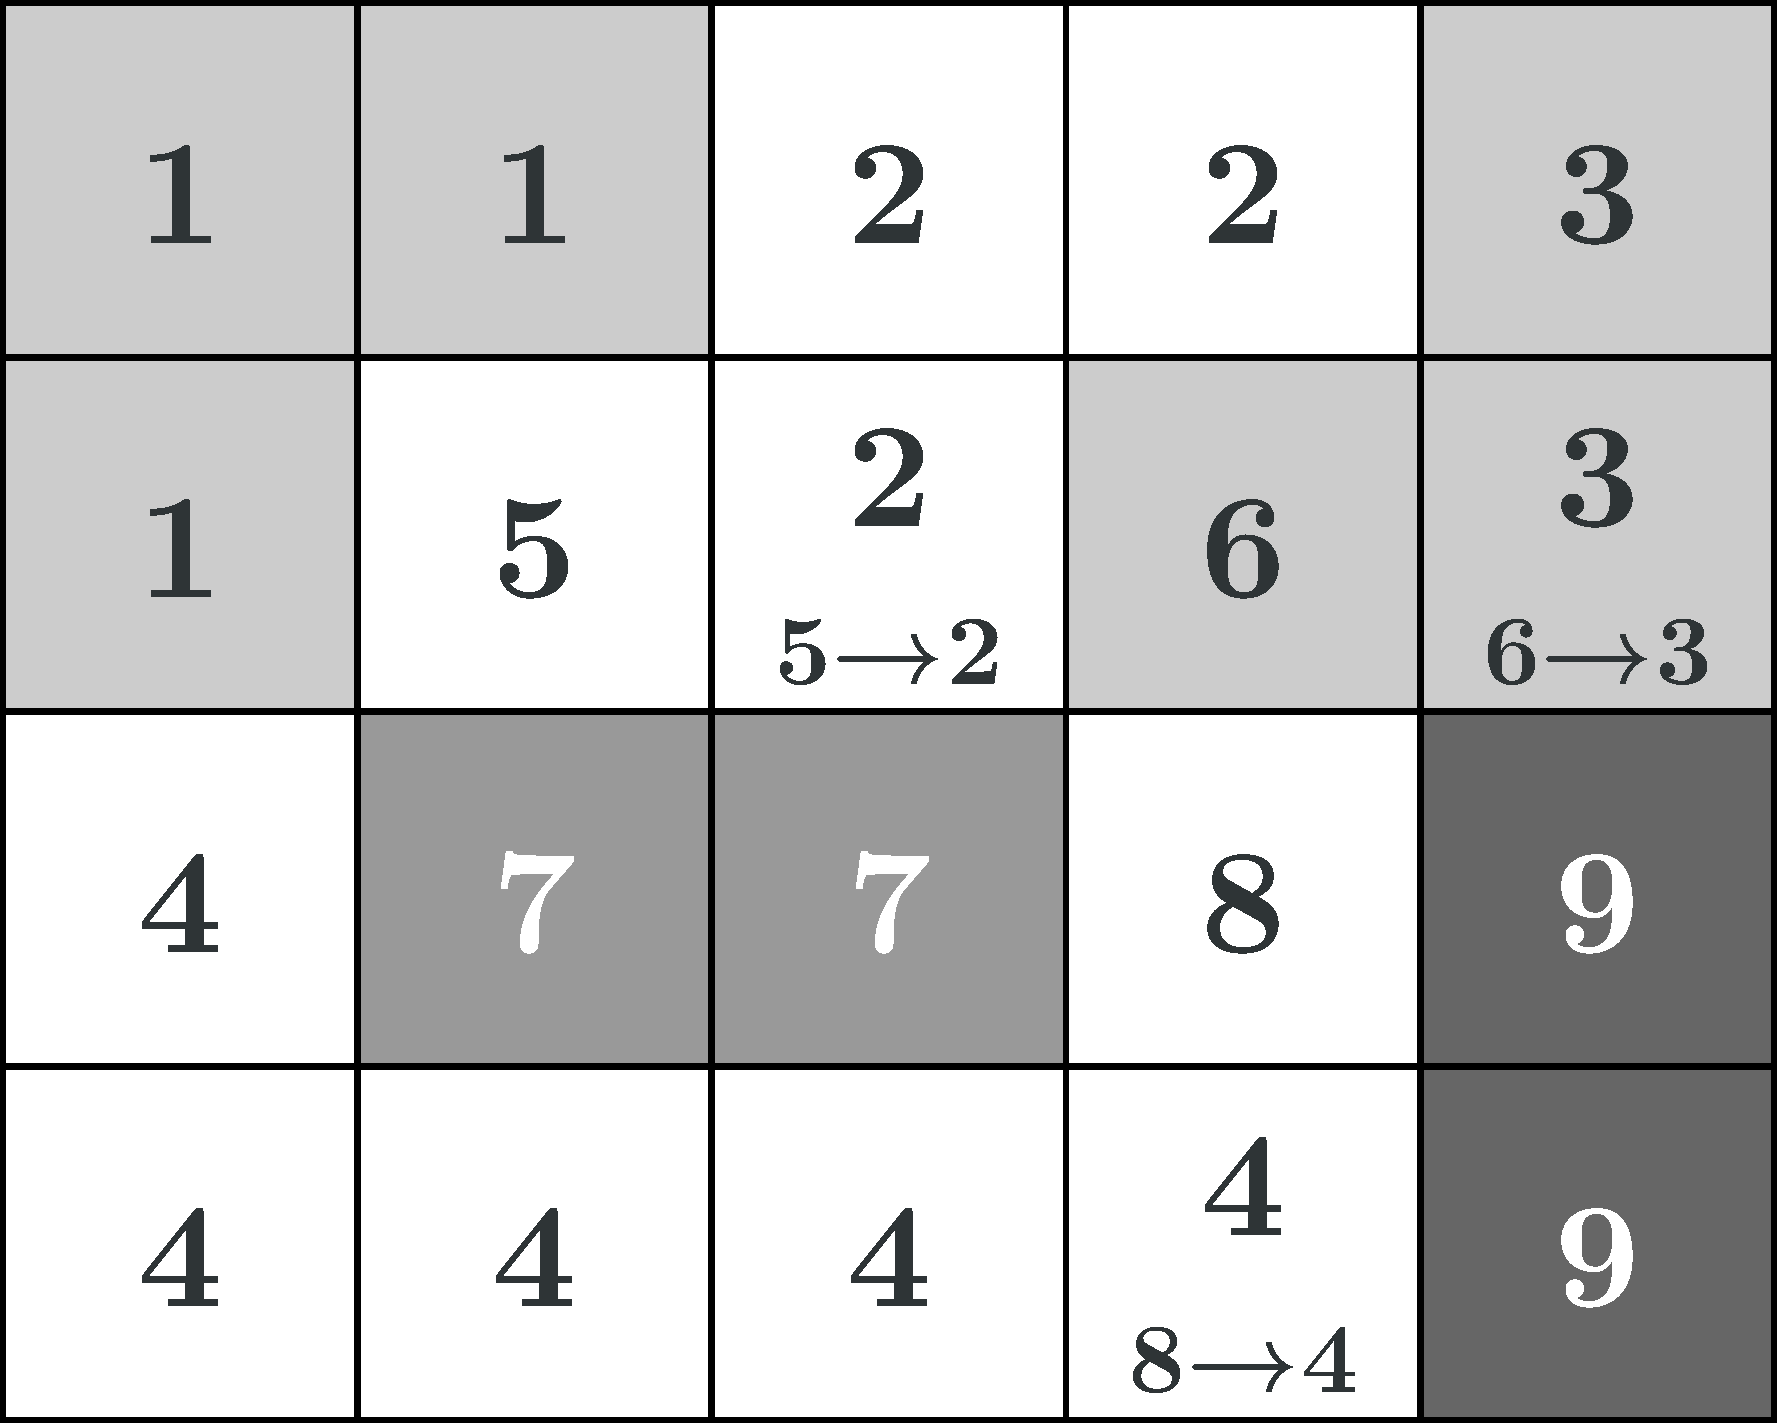
\includegraphics[width=\columnwidth]{img/basics/connected-compontents/labeling-2}
    \caption{Label zuweisen und Äquivalenzen ($\rightarrow$) aufzeichnen}
  \end{subfigure}
  \begin{subfigure}[t]{0.327\columnwidth}
    \centering
    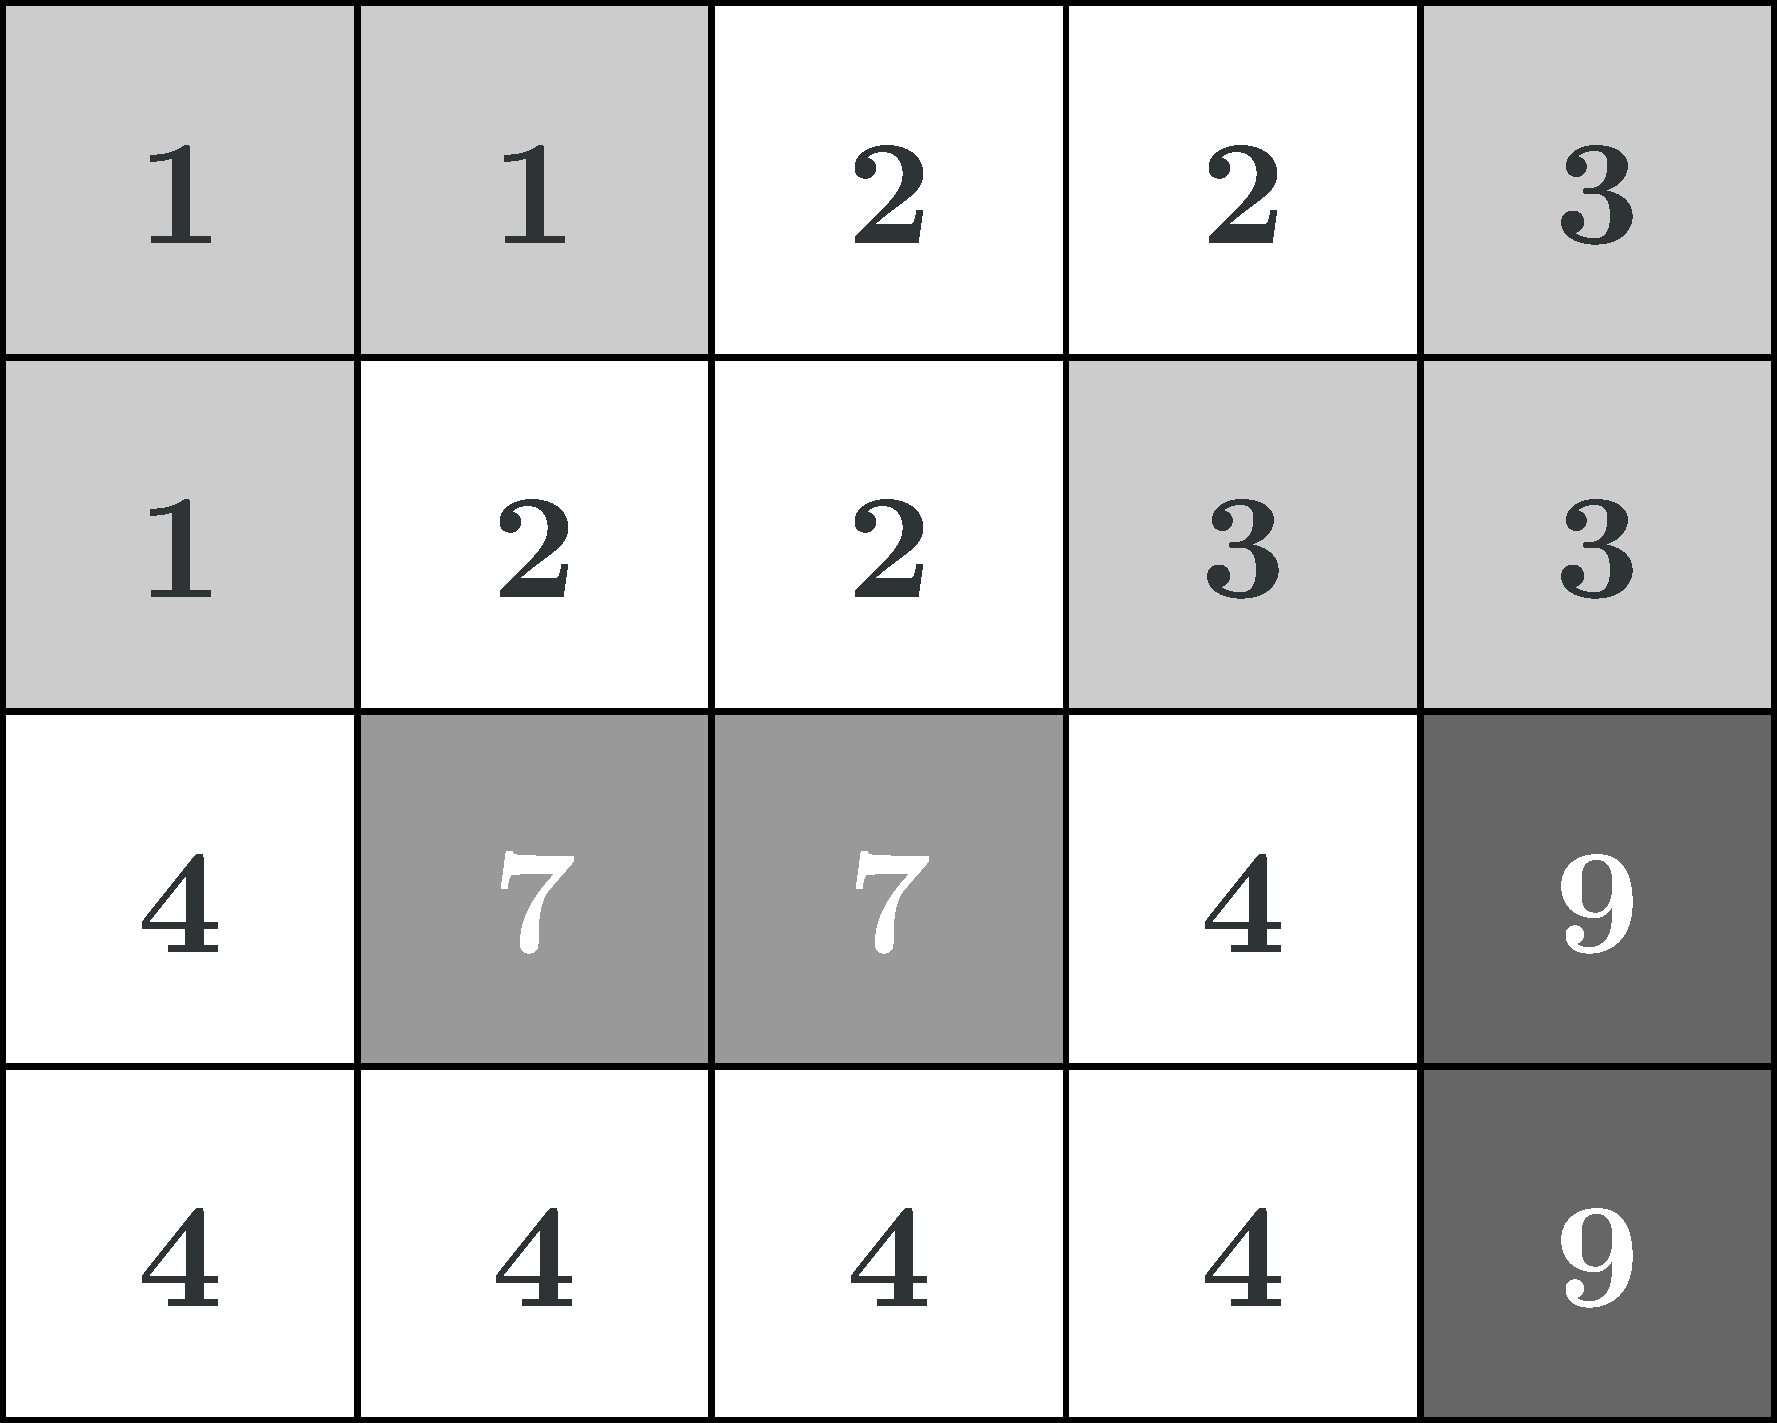
\includegraphics[width=\columnwidth]{img/basics/connected-compontents/labeling-3}
    \caption{Äquivalenzen auflösen}
  \end{subfigure}
  \caption[Ablauf des Connected-Components-Labeling]{Ablauf des Connected-Components-Labeling mit 4-Konnektivität.}
\end{figure}

\section{Konvexe Hülle}
\writtenby{\dcauthornameewie}%
Als konvexe Hülle einer Punktmenge $M$ bezeichnet man das minimale konvexe Polygon, welches sämtliche Punkte aus $M$ enthält.
Für die Berechnung der konvexen Hülle aus einer Menge von Punkten existieren diverse Alogirthmen.
Ein simpler Algorithmus ist \textsc{Andrew}'s Monotone Chain  \cite[6--7]{compgeom2008}.
Dazu werden zwei "`halbe"' Hüllen erstellt, die obere Hülle $U$ und untere Hülle $L$.
Die obere Hülle wird erzeugt indem über alle Punkte der Menge $M$ entsprechend ihrer lexikografischen Ordnung\footnote{
  \( (x,y) < (u, v) \Longleftrightarrow x < u \vee x = u \wedge y < v \)
} iteriert, und wiederholt das letzte Element in $U$ entfernt wird solange $U$ mindestens 2 Punkte enthält und die letzten 2 Punkte zusammen mit dem aktuell betrachteten Punkt \emph{keine} Rechtskurve bilden.
Anschließend wird der aktuelle Punkt ans Ende von $U$ eingefügt.
Die Erzeugung der unteren Hülle $L$ erfolgt analog $U$, jedoch unter Betrachtung der Punkte in umgekehrter Reihenfolge.
Zudem \emph{müssen} die letzten 2 Punkte zusammen mit dem aktuell betrachteten Punkt eine Rechtskurve bilden.
Abschließend werden $U$ und $L$ so zusammen gefasst, dass diese die konvexe Hülle als Liste von Eckpunkten im Uhrzeigersinn ergeben.


\chapter{Strichcodes}
\writtenby{\dcauthornameriren}%
In diesem Kapitel werden erst einige Strichcodes etwas genauer beschrieben und anschließend einige Strichcodegeneratoren und -erkenner vorgestellt.

\section{Einige Strichcodes}
\writtenby{\dcauthornameriren}%
Um die eigentliche Aufgabe etwas genauer zu beleuchten, werden hier 2 unterschiedliche Strichcodearten repräsentativ vorgestellt und ihr Aufbau genauer untersucht.

\input{tex/barcodes/thecodes/code39}
%\input{tex/barcodes/thecodes/code128}
%\input{tex/barcodes/thecodes/ean}
\input{tex/barcodes/thecodes/qr}

\section{Strichcode Bibliotheken}
\writtenby{\dcauthornameriren}%
Im Internet existieren viele verschiedene Bibliotheken zur Generierung und Dekodierung von Strichcodes aller Arten. Deshalb werden hier einige davon aufgeführt und es wird darauf eingegangen, warum ZXing genutzt wird.


\subsection*{Open-Source Strichcode Generatoren}
Um die Strichcodeerkenner testen zu können, ist es nötig einige Strichcodes zu erstellen, um den Funktionsumfang zu überprüfen. Dazu wurden einige Strichcode Generatoren ausgewählt und diese werden hier, für mögliche weitere Tests, kurz vorgestellt.

\paragraph*{Der Barcode Writer}
Der Barcode Writer ist in PostScript geschrieben und kann alle Codeformate erstellen. Er untersteht dabei der 'MIT/X-Consortium License' und kann hier gefunden werden:\\ \url{https://code.google.com/p/postscriptbarcode}

\paragraph*{Barcode4J}
Barcode4J ist in Java geschrieben und kann auch sehr viele Strichcodes generieren, wenn auch nicht so viele wie der Barcode Writer. Barcode4J untersteht dabei der 'Apache Licence v2.0' und genaueres erfährt man hier:\\
\url{http://barcode4j.sourceforge.net/index.html}

\paragraph*{www.terryburton.co.uk}
Unter \url{http://www.terryburton.co.uk/barcodewriter/generator} kann man online jegliche Art von Strichcode generieren und in verschiedenen Dateiformaten (jpg, png, eps) herunterladen, wodurch man die Installation, oder sogar Kompilierung, eines extra Programmes umgehen kann.



\subsection*{Open-source Barcode Scanner}
Für die Erkennung von Strichcodes gibt es einige gute Open-Source Bibliotheken, wobei hier nur die vom genannten Funktionsumfang größten kurz untersucht werden.

\paragraph*{ZXing('Zebra Crossing')}
\label{par:zxing}
Die Bibliothek ZXing('Zebra Crossing') besitzt einen riesigen Funktionsumfang, unter den durch sie unterstützten Codes sind z.B. UPC-A/UPC-E, EAN-8/EAN-13, Code 39, Code 128, ITF, Codabar, RSS-14(alle Varianten), QR Code und Data Matrix. Zusätzlich können diese Strichcodes auch mit ZXing generiert werden. Weiter Pluspunkte sind, dass ZXing in Java geschrieben ist und unter der 'Apache License v2.0' zur Verfügung gestellt wird. Dadurch lässt sie sich nahtlos in die Software der Professur Medieninformatik integrieren. Ihr Quellcode kann hier gefunden werden:\\
\url{http://code.google.com/p/zxing}

\paragraph*{ZBar}
ZBar erkennt auch einen großen Anteil an Strichcodes und ist betriebssystemunabhängig in C geschrieben, wobei es sogar Schnittstellen zu C++, Perl und Python besitzt. Einige der erkannten Codes sind z.B. EAN-13/UPC-A, UPC-E, EAN-8, Code 128, Code 39, Interleaved 2 of 5 and QR Code. ZBar steht unter der 'GNU LGPL 2.1' und mehr Informationen findet man unter:\\
\url{http://zbar.sourceforge.net}.

\paragraph*{BarBara Barcode Library}
BarBara ist ein Strichcodescanner in VB6, VB.NET und PHP5, der ebenso sehr viele Strichcodes unterstützt, wie z.B. Code39, UPC, MSI, 2of5 und Codeabar. Diese Bibliothek ist dabei unter der 'GNU LGPL' verfügbar und weitere Informationen kann man hier finden:\\
\url{http://sourceforge.net/projects/barbara}

\paragraph*{Bewertung}
Die Bibliotheken wurden empirisch getestet und erfüllten alle funktionalen Anforderungen, wodurch die Integration in das Auswertungsprogramm und die Nutzung nach Lizenz die wichtigsten Auswahlkriterien werden. Da ZXing in Java geschrieben ist und unter der 'Apache License v2.0' verfügbar ist, wurde ZXing am Ende als optimal ausgewählt.


\chapter{Entwickelte Verfahren}

\chapter{Auffinden und Extrahieren der Barcodekandidaten}
\writtenby{\dcauthornameewie}%
Um Regionen mit potentiellen Barcodes zu ermitteln machen wir uns den Umstand zu Nutze, dass lesbare Barcodes einen relativ hohen Kontrast aufweisen und sich in dieser Hinsicht von deren Umgebung abheben.

\begin{enumerate}[(i)]
\item \textbf{Graustufen}
\todo[inline,author=\dcauthornameewie]{Konvertierung erfolgt durch Zeichnen des Bildes in ein \texttt{BufferedImage} mit ColorModel \texttt{TYPE\_BYTE\_GRAY} (schnell).
Jedoch ohne Kenntnis der zu Grunde liegenden Formel zur Berechnung des Grauwertes.}

\item \textbf{Kantenbild bestimmen} Das Kantenbild $I_{edge}$ ergibt sich aus der pixelweisen Addition der absoluten Werte zweier Gradientenbilder (in horizontaler und vertikaler Richtung). 
Die beiden Gradientenbilder werden durch Faltung mit dem \textsc{Roberts}-Operator berechnet.
  \[ I_{edge}(x,y) = \big|(I_{lum} \circ K_X)(x,y)\big| + \big|(I_{lum} \circ K_Y)(x,y)\big| \]
Wir verwenden den Roberts-Operator, da dieser sich für unser Problem als ideal erwiesen hat.
\todo[author=\dcauthornameewie]{näher erläutern}

\item \textbf{Kanten verstärken} Die Kanten werden mit einem $5\times5$ Strukturelement mittels Dilation verstärkt.
    \[ I_{edge}^\bullet = I_{edge} \oplus D, \quad D = [-2,2]\times[-2,2] \]

\item \textbf{Segmentierung} Das Kantenbild wird anschließend segmentiert um jedes Pixel entweder dem Vordergrund (Kanten) oder dem Hintergrund zuzuordnen.
Wir nutzen dazu das Schwellwertverfahren.
Als Schwellwert \( t \) dient die mittlere Helligkeit aller Pixel.
  \[ I_{bin}(x,y) = \begin{cases}
       0   & I_{edge}^\bullet(x,y) \leq t \\
       255 & I_{edge}^\bullet(x,y) > t
     \end{cases} \]

\item \textbf{Komponenten extrahieren} Um alle zusammenhängenden Komponente aus $I_{bin}$ zu extrahieren wenden wir das \textit{connected-component labeling} an.
Dabei behandeln wir $I_{bin}(x,y) = 0$ als Hintergrund welcher als eine einzige Komponente mit Label $0$ erfasst wird.
Dadurch kann der Hintergrund leicht verworfen werden, da er für die weitere Verarbeitung nicht von belang ist.

\item \textbf{Regionen klassifizieren} Die extrahierten Komponenten beschreiben bisher nur Bildelemente mit erhöhtem Kontrast.
Darunter fallen, neben den erwünschten Barcodes, auch Elemente wie z.B. Schrift und Symbole.
Um alle potentiellen Barcodes auszuwählen müssen wir alle Komponente herausfiltern welche nicht als Barcode in Frage kommen.
Dazu berechnen wir für jede Komponente deren konvexe Hülle über den Koordinaten der entsprechenden Pixel.

Jetzt können wir für jede Region den Deckungsgrad $\gamma$ definieren, d.h. welchen Anteil die Fläche einer Komponente, d.h. die Anzahl der enthaltenen Pixel, an der Fläche $A$ des Polygons \cite{braden1986} besitzt, das durch die konvexe Hülle beschrieben wird.
  \begin{align*}
    \gamma &= \frac{|C|}{A} \in [0,1]
           & C~\hat=~\text{Punktmenge einer Komponente} \\
         A &= \frac{1}{2} \sum_{i=0}^{n-1}{\hat x_i (\hat y_{i+1} - \hat y_{i-1})}
           & \hat z_i = z_{i \bmod n}
  \end{align*}

\begin{itemize}
  \item Minimum Area Enclosing Rectangle
  \item Axis Aligned Bounding Rectangle
\end{itemize}

\todo[author=\dcauthornameewie]{weitere Maße}

\end{enumerate}

\section{Auffinden potentieller Barcodes}
\writtenby{\dcauthornameewie}%
Um maschinell lesbar zu sein, zeichnen sich Barcodes durch einen, im Vergleich zur ihrer Umgebung, hohen Helligkeitskontrast aus.
Das im Folgenden beschriebene Verfahren macht sich diesen Umstand zu nutze um Bildregionen zu identifizieren, die mit höherer Wahrscheinlichkeit Barcodes enthalten.
Das Verfahren arbeitet mit einem Graustufenbild \autoref{sec:grayscaling}, das die Helligkeit der Pixel kodiert.

\begin{enumerate}[(1)]
\item \textbf{Kantenbild bestimmen}
Das Kantenbild wird gemäß \autoref{sec:edge-detection} ermittelt.
Der \textsc{Roberts}-Operator erweist sich am geeignetsten da er Bildrauschen weniger stark erfasst als z.B. der \textsc{Sobel}-Operator.

\item \textbf{Kanten verstärken}
Die Kanten werden mit einem $5\times5$ Strukturelement mittels Dilation verstärkt.
Dadurch wird erreicht, dass nah beieinander liegende Kanten (wie es bei Strichcodes der Fall ist) eine möglichst geschloßene Fläche bilden.
Hierbei ist die Wahl der Größe des Strukturelements entscheidend.
Ist es zu klein, bleiben zu große Löcher übrig.
Ist es zu groß kann es vorkommen, dass Barcodes mit geringem Abstand zueinander zu einer Fläsche verschmelzen (trotz vorhandener Ruhezone).

\item \textbf{Segmentierung}
Die Segmentierung erfolgt mittels Thresholding.
Als Schwellwert dient der Mittelwert der Helligkeit aller Bildpunkte.
Die Verwendung des Mittelwertes ist ideal, da sich Kantenpixel durch ihren Gradienten bereits deutlich vom Hintergrund abzeichnen.
Das Resultat ist ein Binärbild mit Hintergrund in schwarz (0\%) und Bildelementen in weiß (100\%).

\item \textbf{Komponenten extrahieren}
Wie in \autoref{sec:connected-components} beschrieben, werden die zusammenhängenden Komponenten der Bildelemente extrahiert.
Punktmengen stellen die resultierenden Komponenten dar.

\item \textbf{Regionen klassifizieren}
Die extrahierten Komponenten beschreiben bisher nur Bildelemente mit erhöhtem Kontrast.
Darunter fallen, neben den erwünschten Barcodes, auch Elemente wie z.B. Schrift und Symbole.
Um alle potentiellen Barcodes auszuwählen sind alle Komponente, die nicht als Barcode in Frage kommen, herauszufiltern.

Es hat sich gezeigt, dass Regionen, denen Barcodes entsprechen, sich dadurch auszeichnen, dass deren Komponenten deutlich geschloßener sind (d.h. weniger Löcher besitzen) als andere falsch-positive Regionen und deren Flächen besser abdecken.
Als Maß für die Abdeckung~$\gamma$ dient das Verhältnis der Anzahl der Pixel einer Komponente~$C$ und der Fläche~$A$ \cite{braden1986} ihrer konvexen Hülle.
\begin{align}
  \gamma &= \frac{|C|}{A} \in [0,1] \\
       A &= \frac{1}{2} \sum_{i=0}^{n-1}{\hat x_i (\hat y_{i+1} - \hat y_{i-1})}
         & \hat z_i = z_{i \bmod n}
\end{align}
Der Wertebereich $\gamma\in[0,1]$ ergibt sich aus der Definition der konvexen Hülle, dass diese alle Punkte einschließt über denen sie konstruiert ist.

Neben der Abdeckung ist die Größe einer Region sinnvoll um Regionen ausschließen zu können die zu klein sind um einen lesbaren Barcode zu enthalten.
Unter der Annahme, dass Barcodes rechteckig sind (ShotCode stellt dabei eine Außnahme dar), ist es möglich Breite und Höhe über ein, die konvexe Hülle umschließendes, Rechteck mit minimaler Fläche zu bestimmen.
Dieses Rechteck, auch "`minimum area enclosing rectangle"' genannt, lässt sich mittels Rotating Calipers berechnen~\cite{arnon1983}.
Da die meisten Barcodes breiter als hoch sind (Ausnahmen sind quadratische Barcodes wie z.B. QR Code oder Data Matrix), ist es möglich die Orientierung anhand dieses Rechtecks zu bestimmen.
\end{enumerate}

%\renewcommand{\thesubfigure}{\scriptsize\alph{subfigure}}

\begin{figure}[H]
  \centering
  \begin{subfigure}[t]{.32\columnwidth}
    \centering
    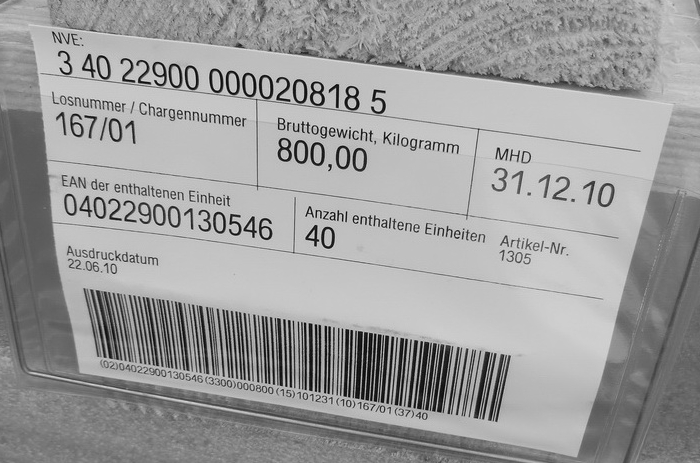
\includegraphics[width=\columnwidth]{img/techniques/candidate-extraction/grayscale}
    \caption{\scriptsize Grauwerte}
  \end{subfigure}
  \begin{subfigure}[t]{.32\columnwidth}
    \centering
    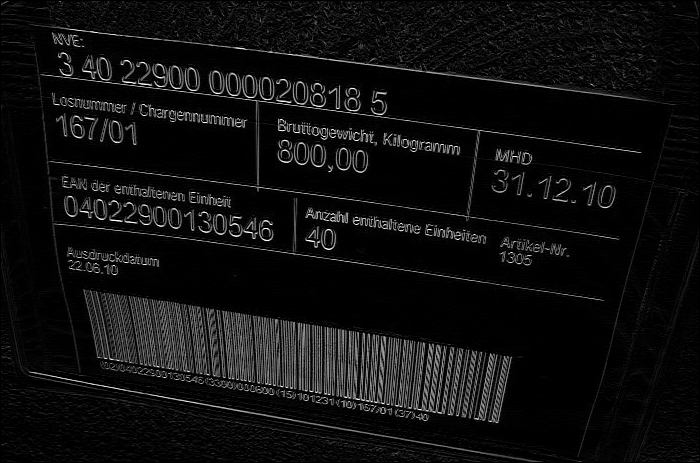
\includegraphics[width=\columnwidth]{img/techniques/candidate-extraction/edges}
    \caption{\scriptsize Kantenbild unter Verwendung des \textsc{Roberts}-Operator}
  \end{subfigure}
  \begin{subfigure}[t]{.32\columnwidth}
    \centering
    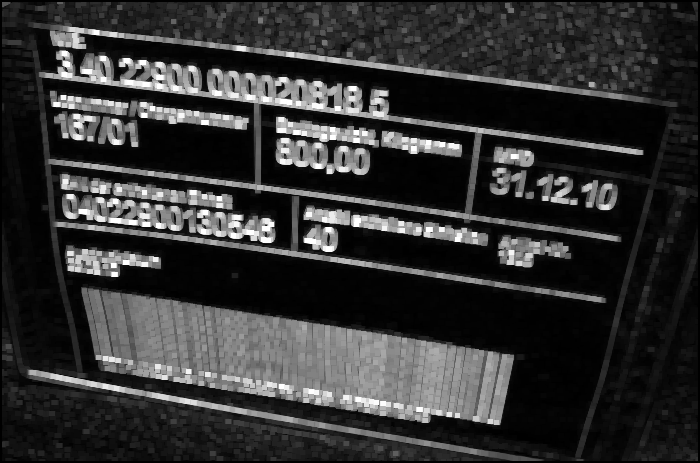
\includegraphics[width=\columnwidth]{img/techniques/candidate-extraction/dilation}
    \caption{\scriptsize Dilation mit einem 5$\times$5-Strukturelement}
  \end{subfigure}
  \begin{subfigure}[t]{.32\columnwidth}
    \centering
    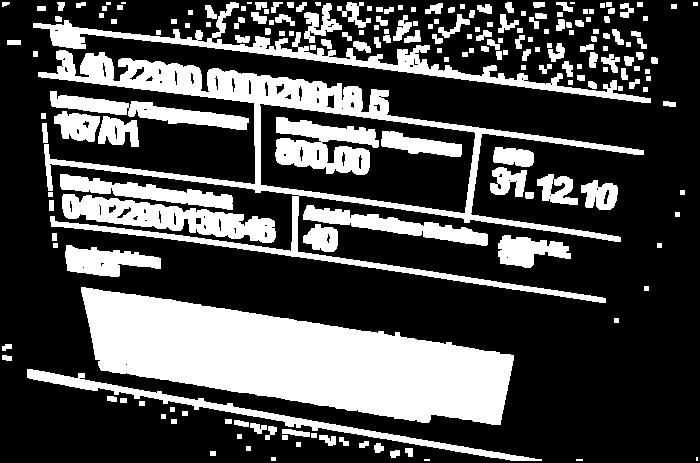
\includegraphics[width=\columnwidth]{img/techniques/candidate-extraction/binary}
    \caption{\scriptsize Binärbild}
  \end{subfigure}
  \begin{subfigure}[t]{.32\columnwidth}
    \centering
    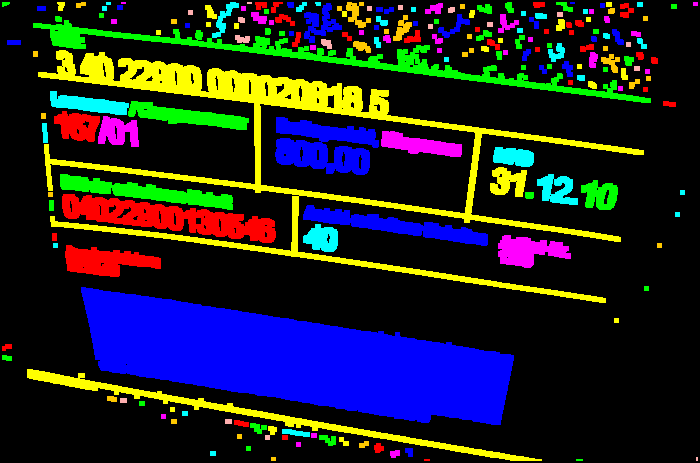
\includegraphics[width=\columnwidth]{img/techniques/candidate-extraction/components}
    \caption{\scriptsize zusammenhängende Komponenten farblich hervorgehoben}
  \end{subfigure}
  \begin{subfigure}[t]{.32\columnwidth}
    \centering
    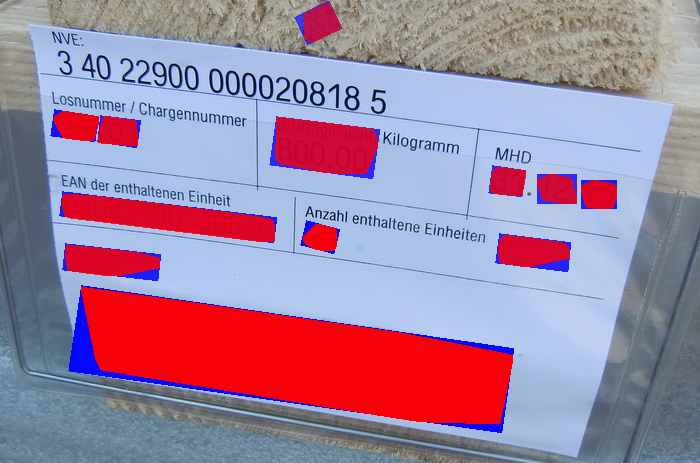
\includegraphics[width=\columnwidth]{img/techniques/candidate-extraction/candidates}
    \caption{\scriptsize ermittelte Regionen (rot) mit umschließendem Rechteck minimaler Fläche (blau)}
  \end{subfigure}
  \caption[Einzelschritte beim Auffinden potentieller Barcodes]{
    Einzelschritte beim Auffinden potentieller Barcodes in einem Bild\protect\footnotemark.
    Bild (f) zeigt deutlich, dass das Verfahren auch Text erfasst.}
\end{figure}

\footnotetext{\url{http://commons.wikimedia.org/wiki/File:Drahtb\%C3\%BCgeltasche_A6.jpg}}




\chapter{Implementierung}
Dieses Kapitel widmet sich der Beschreibung der wesentlichen Aspekte der Implementierung.
Dazu ist nicht jede einzelne Funktion aufgeführt, sondern nur die wichtigsten, die für das Verständnis der Verarbeitung erforderlich sind.

Das Diagramm in \autoref{fig:uml0} zeigt die Beziehungen zwischen den zentralen Komponenten der Implementierung, auf die im Folgenden einzeln eingegangen wird.
Aus Platzgründen sind die Klassendiagramme nur auf öffentliche sowie geschützte Methoden beschränkt.
Klassen, die lediglich eine Abhängigkeit darstellen und nicht Bestandteil einer Bibliothek sind, werden nur mit ihrem Namen dargestellt.
\elasticfigure[fig:uml0]{img/uml/uml.0}{zentrale Komponenten der Implementierung und deren Beziehungen untereinander}

\section{Klasse \code{Job}}
Die Klasse \code{Job} kapselt die Bildquelle~(Methode \code{getSource}) und erzeugt fortlaufend nummerierte Extractions~(Methode \code{createExtraction}).
Zudem stellt es für die Extractions ein URL Template~(Methode \code{getExtractionUrlTemplate}) zur Verfügung um jeder Extraction eine URL zuzuordnen die zur Speicherung der Extraction nötig ist.
Durch die Initialisierung eines Jobs mit einer optionalen Framenummer~(Parameter \code{initialFrameNumber}) ist es möglich die Verarbeitung eines Jobs an einer gewünschten Stelle wieder fortzusetzen.

\elasticfigure{img/uml/uml.115}{Klassendiagramm von \code{Job}}


\section{Klasse \code{Extraction}}
Eine Instanz der Klasse \code{Extraction} kapselt alle Regionen~(\code{getRegions()}) und Barcodes~(\code{getBarcodes()}) die aus genau einem Bild extrahiert wurden.
Jede Instanz trägt, beginnend bei 0, die Nummer des entsprechenden Frames des Quellmaterials~(\code{getFrameNumber()}).
Die Barcodes einer Extraction sind in zwei Kategorien unterteilt.
\begin{itemize}
  \item gebundene Barcodes~(\code{getRegionBarcodes()}), die von einer Region erfasst sind
  \item ungebundene Barcodes~(\code{getRegionlessBarcodes()}), die von keiner Region erfasst sind
\end{itemize}

\elasticfigure{img/uml/uml.110}{Klassendiagramm von \code{Extraction}}


\section{Klasse \code{Region}}
Instanzen der Klasse \code{Region} beschreiben Bildregionen.
Als Grundlagen dienen z.B. die zusammenhängenden Komponenten eines Bild.
Eine Region ist durch ein konvexes Polygon~(Methode \code{getConvexPolygon}) und einen Deckungsgrad~(Methode \code{getCoverage}) beschrieben.
Die Methode \code{getOrientedRectangle} erzeugt aus dem konvexen Polygon das umschließende Rechteck mit minimaler Fläche.
Im Gegensatz dazu erzeugt die Methode \code{getAxisAlignedRectangle} das achsenparallele Rechteck.

\elasticfigure{img/uml/uml.116}{Klassendiagramm von \code{Region}}


\section{Klasse \code{Barcode}}
Die Klasse \code{Barcode} dient der Beschriebung erfolgreich gelesener Barcodes.
Ein Barcode besteht aus seinem Typ~(\code{getType()}), dem kodierten Text~(\code{getText()}), den Binärdaten~(\code{getBytes()}) sowie mehreren Punkten~(\code{getAnchorPoints()}), die zum Lesen des Barcodes dienten.
Die Punkte können z.B. der Start- und Endpunkt der Scanline für einen eindimensionalen Barcode sein oder die Mittelpunkte der Marker bei einem zweidimensionalen Barcode~(z.B. QR Code).

\elasticfigure{img/uml/uml.101}{Klassendiagramm von \code{Barcode}}


\section{Klasse \code{Source}}
Das Klasse \code{Source} stellt eine Bildquelle dar, die ein Objekt erzeugen kann welches Bilder bereitstellt~(\code{createImageProvider()}).
Eine konkrete Bildquelle kapselt dazu die Informationen die zur Erzeugung einer Bildquelle nötig sind (z.B. die URL einer Videoresource).

\elasticfigure{img/uml/uml.119}{Klassendiagramm von \code{Source}}

\subsection*{Konkrete Implementierungen}
Insgesamt existieren 6 Realisierungen von \code{Source} die sich im Laufe der Entwicklung als sinnvoll erwiesen haben.
Die Klasse \code{SourceFactory} stellt Factory-Methoden zu Verfügung um die hier gelisteten Implementierungen zu erzeugen.

{
\setlength{\leftmargini}{1.5em}
\setlength{\labelsep}{\textwidth}
\begin{description}
  \item[\code{BufferedImageSource}]
    Verwendet eine geordnete Sammlung von \code{BufferedImage}-Instanzen.
    Diese Klasse ist sinnvoll wenn die Bilder bereits von einer Anwendung geladen sind.
  \item[\code{ImageCollectionSource}]
    Verwendet eine Liste von URLs um Bilder lokal oder aus einem Netzwerk (z.B. über HTTP) zu laden.
  \item[\code{ImageSequenceSource}]
    Verwendet eine URL um durchnummerierte Bilder (ebenfalls lokal oder aus einem Netzwerk) zu laden.
    Ein Anwendungsfall ist z.B. Bilder die zuvor bereits aus einem Video extrahiert wurden und daher durchnummeriert vorliegen.
  \item[\code{ImageSnapshotServiceSource}]
    Verwendet eine URL für einen Webservice, der bei jedem Request ein neues Bild liefert (z.B. eine Netzwerkwebcam).
  \item[\code{VideoDeviceSource}]
    Nutzt eine Videogerät, welches über eine Zahl, beginnend bei 0, identifiziert wird.
    Zum Lesen der Videodaten dient JavaCV\footnote{\url{http://code.google.com/p/javacv/}} um auf die C/C++-API von OpenCV\footnote{\url{http://opencv.org}} zugreifen zu können.
  \item[\code{VideoFileSource}]
    Verwendet eine URL zum laden eines Videos, welches lokal aber auch in einem Netzwerk (Zugriff über HTTP) vorliegen kann.
    Nutzt ebenfalls JavaCV zum Lesen der Daten.
\end{description}
}


\section{Klasse \code{Extractor}}
Der \code{Extractor} stellt die Implementierung des in \autoref{sec:extraction} beschriebenen Verfahrens.
Als Eingabe dient eine Instanz von \code{Job}.
Die Verarbeitung der Bilder erfolgt sequentiell durch wiederholten Aufruf der Methode \code{processNextImage}.
Dem, mit der Methode \code{setExtractionHandler} gesetzten, \code{ExtractionHandler} werden nach jedem verarbeiteten Bild die erzeugte \code{Extraction}-Instanz sowie das entsprechende Bild übergeben.

Die einzelnen Verarbeitungsschritte des Extractors sind über Interfaces realisiert, wodurch es möglich ist das Verfahren durch alternative Implementierungen anzupassen.
Das Grauwertbild wird mittels eines \code{Grayscaler}~(Methode \code{setGrayscaler}) bestimmt.
\code{RegionExtractor}~(Methode \code{setRegionExtractor}) ist für das Auffinden von Regionen zuständig.
Mit \code{Filter<Region>}~(Methode \code{setRegionFilter}) ist es möglich Regionen nach bestimmten Kriterien~(Größe, etc.) auszuwählen.
Für jede gewählte Region wird mit einem \code{ImageEnhancer}~(Methode \code{setImageEnhancer}) der entsprechende Bildausschnitt bildtechnisch aufbereitet.
Abschließend erfolgt unter Verwendung eines \code{BarcodeReader}~(Methode \code{setBarcodeReader}) das Lesen des Barcodes im Bildausschnitt einer jeden Region sowie im gesamten Bild.

\elasticfigure{img/uml/uml.109}{Klassendiagramm von \code{Extractor}}

\input{tex/classes/extractor/grayscaler}
\input{tex/classes/extractor/regionextractor}
\input{tex/classes/extractor/imageenhancer}
\input{tex/classes/extractor/barcodereader}


\section{Serialisierung}
Um Jobs und Extractions speichern und zwischen Anwendungen austauschen zu können ist eine Serialisierung, d.h. die Übersetzung von Objekten in eine maschinenlesbare Form sowie die Wiederherstellung jener Objekte, erforderlich.

XML stellt für diesen Zweck die ideale Lösung dar, da es ein weit verbreiteter Standard zur externen Repräsentierung von Daten darstellt.
Zudem wird an der Professur Medieninformatik im Bereich Informationretrieval bereits die XML-Datenbank eXist\footnote{\url{http://www.exist-db.org/}} eingesetzt wodurch eine XML-Lösung naheliegend erscheint.
Zusammen mit einem XML Schema (siehe \autoref{annex:xml-schema}) ist es möglich die Serialisierung weitesgehend zu automatisieren, da Werkzeuge existieren (z.B. JAXB für Java) die aus einem XML Schema Quellcode erzeugen, der die Serialisierung realisiert.

Die Grundlage der XML-Serialisierung bildet die abstrakte Klasse \code{XmlSerialzer}, die wiederum eine Realisierung des Interface \code{Serializer} ist.
Konkrete Serialisierer wie z.B. \code{XmlJobSerializer} für \code{Job} und \code{XmlExtractionSerializer} für \code{Extraction} müssen ein Objekt des entsprechenden Typs auf ein XML-Element abbilden (Methode \code{createRootElement}) bzw. aus einem XML-Element ein Objekt wieder herstellen (Methode \code{restoreModel}).
Neben Zeichenketten und Bytestreams als Ein- und Ausgabe bietet \code{XmlSerializer} zusätzlich DOM-Knoten als Quelle und Ausgabe.

Optional kann \code{XmlSerializer} die Eingabe bzw. Ausgabe validieren, indem mit der Methode \code{setSchema} das XML Schema gesetzt wird.
Das Schema kann auch über eine URL mittels der Methode \code{setSchemaLocation} verwendet werden.
Ist die URL des Schemas bekannt, so kann diese bei der Serialisierung mit ausgegeben\footnote{\url{http://www.w3.org/TR/xmlschema-1/\#xsi_schemaLocation}} werden.
Die Methode \code{setUrlContext} setzt den URL-Kontext um relative URLs (z.B. relative Dateipfade) auflösen zu können.

\elasticfigure{img/uml/uml.150}{Klassendiagram von \code{XmlSerialzer}}



\section{Klasse ImageProcessing}
\writtenby{\dcauthornameriren}%
Das Ziel dieser Klasse ist es, einzelne Eigenschaften von Strichcodebilder so aufzuwerten, dass der enthaltene Strichode besser von der Bibliothek ZXing erkannt werden kann.
Zusätzlich sind auch noch einige weitere Funktionen implementiert, die teilweise andere Varianten oder einfach zusätzliche Funktionen darstellen. Auf diese wird hier aber nicht näher eingegangen, da sie keinen direkten Bezug zur aktuellen Implementation haben. Sie wurden aber nicht aus der Klasse entfernt, um die mögliche spätere Weiterentwicklung zu erleichtern.

Die Bildverarbeitung erfolgt mittels ImageJ\footnote{\url{http://rsbweb.nih.gov/ij/}}, ein gemeinfreies (public domain) Bildbearbeitungsprogramm, dessen Bibliotheken ebenfalls frei nutzbar sind.

\elasticfigure{img/uml/uml.127}{Klassendiagramm von \code{ImageProcessing}}

\subsection*{Methode hasShade}
Diese Methode erhält ein Eingabebild, überprüft ob es Schatten enthält und gibt einen Wahrheitswert als Antwort zurück.
Die möglichen Schatten werden über den weißen Rand der Strichcodes gesucht. Wenn dort ein ausreichend großer Helligkeitsunterschied auftritt, wird angenommen, dass es einen Schatten gibt, der nicht mehr von ZXing erkannt werden kann.
Um die Erkennung möglichst variabel zu gestalten, wurde zusätzlich ein Faktor für die Genauigkeit der Erkennung eingeführt. Er bestimmt die Anzahl an Pixeln, die, pro Seite, in die Untersuchung aufgenommen werden.
Die Voraussetzung für die korrekte Funktionsweise der Methode ist, dass die Ruhezone, um den Strichcode, nicht überlagert wird. Die Schattenerkennung wäre durch andere Objekte in dieser Zone korrumpiert, da durch diese definitiv die Helligkeitsunterschiede in diesem Bereich zu stark beeinflusst würden.


\subsection*{Methode isBlurry}
Diese Methode erhält ein Eingabebild und gibt einen Grad an Unschärfe für dieses zurück.
Das Bild wird dafür mit einem Laplacian-of-Gaußian-Filter bearbeitet und dadurch wird ein Bild erhalten, indem, wie in Kapitel \ref*{sec:LoG} beschrieben, der größte Wert die Schärfe der Abbildung repräsentiert.
Der Ausgabewert ist allerdings abhängig von der allgemeinen Helligkeit des Bildes, daher sollte ein bereits normalisiertes Bild als Eingabe dienen.


\subsection*{Methode isDark}
Diese Methode erhält ein Eingabebild und errechnet die ungefähre Helligkeit des Eingabebildes.
Die Helligkeit wird durch ein Histogramm bestimmt, indem aus ihm der Durchschnittswert (wo die Hälfte aller Pixel heller bzw. dunkler sind) berechnet wird. Dabei entsprechen kleinere Werte mehr dunklen Pixeln.


\subsection*{Methode isRotated}
Diese Methode erhält ein Eingabebild und gibt den Rotationswinkel des enthaltenen Strichcodes zurück.
Um den Winkel zu bestimmten, werden vom linken Rand aus starke Helligkeitsunterschiede gesucht und diese gefundenen Punkte werden, von oben nach unten, in einem Array gespeichert. Danach wird überprüft, ob eine Gerade, durch zwei hintereinander liegende Punkte, auch relativ nah an einem dritten, darauf folgenden Punkt vorbei geht. Wenn ja, dann werden weitere Punkte mit dieser Geraden überprüft und so die Anzahl an Punkten auf ihr bestimmt. Die Gerade mit der maximalen Anzahl an Punkten sollte theoretisch dem Anfangs- oder Endstrich des Codes entsprechen.
Diese Methode ist zwar für 1D Strichcodes konzipiert, funktioniert aber nichtsdestotrotz auch für 2D Codes, da immer eine längere Linie am Rand gefunden werden kann.
Dieser Winkelbestimmung ist nicht exakt, aber reicht für die Erkennung durch die Bibliothek ZXing vollkommen aus, da Abweichungen von maximal 2$ \circ $ nicht ins Gewicht fallen.
 

\subsection*{Methode brightenBufferedImage\_linear}
Diese Methode erhält ein Eingabebild und einen Aufhellungsfaktor, der die Verstärkung der Beleuchtung angibt. Dadurch wird eine hellere bzw. dunklere Variante vom Bild zurückgegeben.
Zum Aufhellen oder entsprechenden Verdunkeln wird ein 'RescaleOp'-Filter genutzt, der entsprechend der pixelbasierten Bildverbesserung funktioniert. Durch ihn wird das Bild vom Normalzustand (Helligkeit=1.0) in einen aufgehellten (Helligkeit>1.0) bzw. abgedunkelten (Helligkeit<1.0) Zustand überführt (plus einem Offset von 15).
Dadurch entsteht eine gleichmäßige Aufhellung des ganzen Bildes.
Eine zweite, realistischere, Variante kann mit einem 'LookupTable'-Filter erzeugt werden, durch den das Bild vom Normalzustand durch eine Helligkeitszuweisung
($newPixelColor = ((oldPixelColor/255.0) * 255.0)^2$)zu jedem Pixel aufgehellt wird.
Dadurch entsteht eine realistische Aufhellung, da dunkle Pixel schneller hell werden. Dies entspricht aber nicht den Anforderungen, da die dunklen Teile für die Erkennung am wichtigsten sind. (Diese Funktion ist trotzdem für mögliche spätere Nutzung als brightenBufferedImage\_quadratic implementiert)


\subsection*{Methode findShades}
Diese Methode erhält ein Eingabebild und gibt das von möglichst allen Schatten befreite Bild zurück.
Die grundsätzliche Idee ist, die Kanten von Schatten zu finden und dann entsprechend den eingerahmten Bereich entsprechend aufzuhellen.
Nach der Implementierung ist allerdings klar geworden, dass der 'BackgroundSubtracter' von ImageJ dies bereits sehr gut tut.
Es wurde auch der Canny-Edge-Detector probiert, allerdings werden dabei zu viele mögliche Kanten erkannt. Also müsste für jedes Bild ein Schwellwert eingestellt werden, wodurch er sich als nutzlos erwies.


%\subsection*{Methode interpolateBufferedImage}
%Diese Methode erhält ein 'BufferedImage' und hellt einen viereckigen Bereich im Bild auf, welcher dann in einem anderen 'BufferedImage' zurückgegeben wird.
%
%Hellt einen Vier-/(Viel-)eckigen Teilbereich auf


\subsection*{Methode rotateBufferedImage}
Diese Methode erhält ein Eingabebild und gibt eine, um den angegebenen Winkel, gedrehte Variante davon zurück.
Das Bild wird über eine affine Transformation gedreht und dann der darzustellende Bereich angepasst.


\subsection*{Methode sharpenBufferedImage}
Diese Methode erhält ein Eingabebild und gibt eine schärfere Variante davon zurück.
Für die Schärfung wird die Methode der unscharfen Maskierung genutzt, wie sie in Kapitel \ref*{sec:unsharp} beschrieben wird.

\section{Klasse ImproveImage}
\writtenby{\dcauthornameriren}%
Das Ziel dieser Klasse ist es, einzelne Eigenschaften von Strichcodebilder so aufzuwerten, dass der enthaltene Strichode besser von der Bibliothek ZXing erkannt werden kann.
Dabei werden die einzelnen Methoden aus der Klasse ImageProcessing zusammen genutzt, um eine optimale Verbesserung der Bilder zu erreichen.

\elasticfigure{img/uml/uml.126}{Klassendiagramm von \code{ImproveImage}}

\subsection*{Methode checkBrightness}
Diese Methode erhält ein Eingabebild, überprüft ob es zu dunkel ist und hellt es wenn nötig auf.
Durch die Methode 'isDark', aus ImageProcessing, wird die Helligkeit des Bildes bestimmt und wenn diese unter der Hälfte der maximalen Helligkeit ist, dann wird sie bis dorthin, durch 'brightenBufferedImage\_linear', aufgehellt.
Nach der Aufhellung werden einige, nur leicht unscharfe, Bilder bereits nutzbar und der Kontrast wird für die spätere Verarbeitung verstärkt.


\subsection*{Methode checkBlur}
Diese Methode erhält ein Eingabebild, überprüft ob es zu unscharf ist und schärft es wenn nötig.
Durch die Methode 'isBlurry', aus ImageProcessing, wird die Schärfe des Bildes bestimmt und wenn diese unter 200 ist, dann wird sie durch 'sharpenBufferedImage' geschärft.


\subsection*{Methode checkRotation}
Diese Methode erhält ein Eingabebild, überprüft wie stark der enthaltene Strichcode gedreht ist und rotiert ihn wieder in eine lesbare Position.
Durch die Methode 'isRotated', aus ImageProcessing, wird der Rotationswinkel des Strichcodes bestimmt und dann wird das Bild durch 'rotateBufferedImage' gedreht.


\subsection*{Methode checkShadow}
Diese Methode erhält ein Eingabebild, überprüft ob Schatten enthalten sind und wenn ja, entfernt diese aus dem Bild.
Durch die Methode 'hasShade', aus ImageProcessing, wird überprüft, ob das Bild Schatten enthält und entfernt sie, wenn nötig, durch 'findShades' aus dem Bild.
 

\subsection*{Methode checkImage}
Diese Methode erhält ein Eingabebild und verbessert es so gut es geht.
Dabei wird als erstes die Helligkeit überprüft ('checkBrightness'), da sie nur positive Auswirkungen auf die folgenden Untersuchungen hat.
Darauf folgt die Untersuchung auf Schatten~('checkShadow'), da diese schlecht auf Umgebungen um den Strichcode reagiert und durch die Rotation möglicherweise ein Rahmen entstehen kann.
Als nächstes wird das Bild rotiert ('checkRotation'), weil dies vor dem Schärfen passieren muss, da das Bild durch die Rotation immer etwas unschärfer wird.
Der letzte Punkt ist dann die Schärfung ('checkBlur').


\chapter{Evaluierung der Ergebnisse}

\section{ZXing}

\input{tex/evaluation/zxing/intro}

\input{tex/evaluation/zxing/ean13}
\input{tex/evaluation/zxing/qr}

\section{Nach der Bildaufbereitung}
\writtenby{\dcauthornameriren}%
Trotzdem die Bibliothek ZXing bereits einen großen Funktionsumfang bereit stellt, enthält sie nichtsdestotrotz Schwachpunkte. Diese werden vor allem bei starker Unschärfe, starken Rotationen und Schatten sichtbar.
Bei der Aufbereitung der Codes wurde daher auf diese Punkte ein besonderes Augenmerk gelegt.

\subsection*{Unschärfe}
\todo{Beschreibung fehlt noch}



\subsection*{Rotation}
Da die Rotation von Strichcodes sich als großes Problem für den Dekodierer herausstellte, wurden Funktionen zur Berechnung des Drehwinkels und der Rotation des Bildes erstellt. Durch diese können alle Strichcodes auf einen erkennbaren Winkel rotiert werden und so mit Sicherheit erkannt werden.

Da aber vor der Erkennung nicht klar ist, um welche Art von Code es sich handelt, wird einfach jeder rotiert, da die Funktionen auch ausreichend gut für andere Codes funktionieren und z.B für QR-Codes die Rotation auch weniger Bedeutung für die Akzeptanz hat.

Problematisch ist es nur, wenn ein Strichcode um 90$ \circ $ gedreht ist, da dann keine durchgehende Gerade wahrnehmbar ist. Allerdings gibt es da die Möglichkeit zwei Durchläufe der Funktionen durchzuführen, da dann erst ein beliebiger anderer Winkel erzeugt wird und beim zweiten Mal richtig rotiert wird.



\subsection*{Schatten}
\todo{Beschreibung fehlt noch}



%\subsection*{Schrägen}




\cleardoublepage
\begin{appendix}
\chapter{XML Schema}
\lstinputlisting[language=XSD]{../core/etc/barcd.xsd}

\end{appendix}


\end{document}
